\chapter*{Introduction}
\addcontentsline{toc}{section}{\textit{Introduction}}
\markboth{\textit{Introduction}}{\textit{Introduction}}

\lettrine{\libertineInitialGlyph{T}}{he} space of knots is the disconnected space of embeddings of \(\S^{1}\) into \(\R^{3}\), in which the connected components, the ``rooms'', are the knot types. Vassiliev studied the space of knots by looking at its ``walls'' of a specific type: those immersions of \(\S^{1}\) into \(\R^{3}\) which fail to be embeddings by having a single point of trasverse intersection. The addition of these walls makes the space of objects we study a connected space. Any two knots are connected by a path that passes through finitely many of the walls. The space of just the walls is also disconnected, but it can be connected by allowing paths to pass through finitely many ``cornices'' where two walls meet. These are immersions that fail to be embeddings by having two points of transverse intersection. The cornices are again disconnected but can be connected by ``corners'' and so on, with any two immersions with \(m\) double points being connected by a path through some finite number of immersions with \(m + 1\) double points.

This constructs the ``stratification'' of the space of knots: a very schematic illustration is given below. Note that this illustration doesn't properly capture the infinite-dimensional nature of the stratification. Nor some other missing details which will appear in Chapter \ref{ch:vassiliev-invariants-and-chord-diagrams}.

\begin{center}
	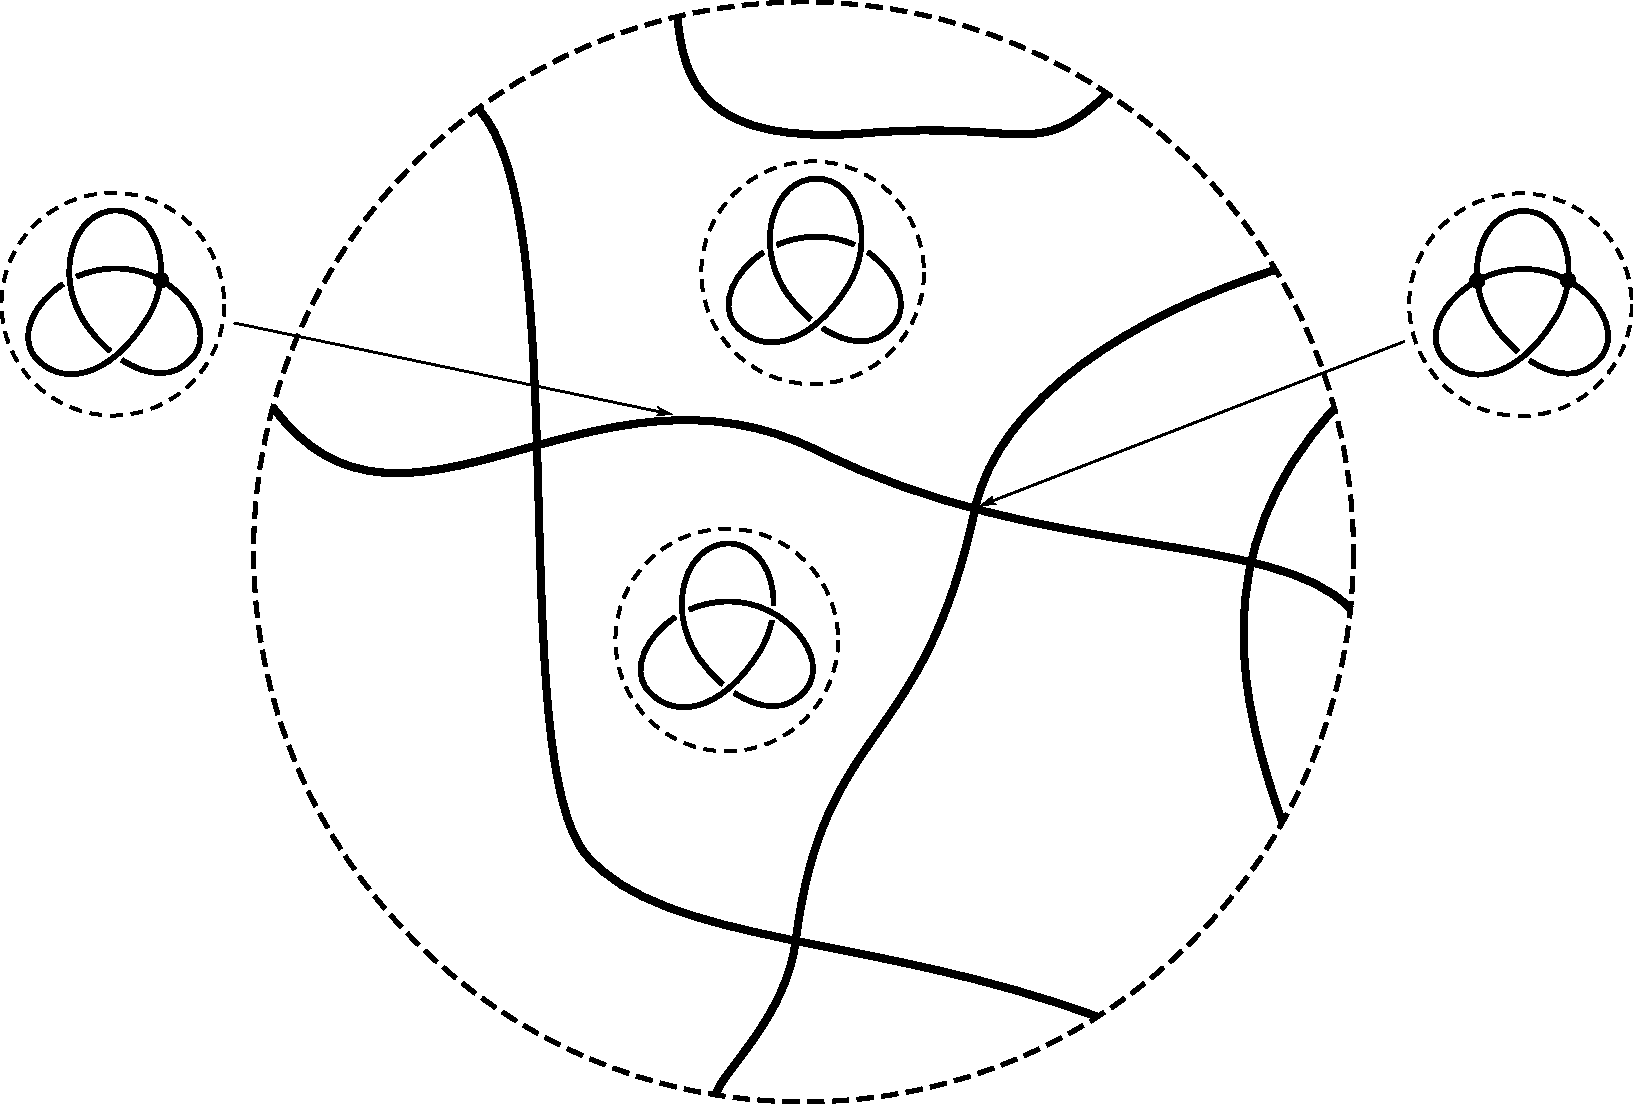
\includegraphics[width=0.55\linewidth]{stratification.pdf}
\end{center}

\begin{mdframed}
	In \cite{cohomology-of-knot-spaces}, Vassiliev makes a sequence of approximations of the cohomology ring of the space of knots, yielding a certain subring of the zeroth cohomology ring. Elements of the zeroth cohomology are locally constant functions on the space, so knot invariants. The invariants in this ``Vassiliev'' subring can be computed on any knot by some procedure involving the homology group of the strata at a finite number of increasing depths.

	Birman and Lin in \cite{knot-polynomials-and-vassilievs-invariants} give an axiomatic definition of the Vassiliev invariants as those that respect the Vassiliev skein relation. It follows, as we will see in Chapter \ref{ch:vassiliev-invariants-and-chord-diagrams} that Vassiliev invariants can be described completely combinatorially by functions on chord diagrams obeying certain combinatorial rules.

	By the work of Bar-Natan in \cite{on-the-vassiliev-knot-invariants} the algebra of chord diagrams turns out to be equivalent to a different diagrammatic algebra, that of Jacobi diagrams, again up to a different set of combinatorial rules. This will be discussed in Chapter \ref{ch:lie-theory-and-jacobi-diagrams}. This change of perspective introduces Lie theory in the following sense. A key relation in the algebra of Jacobi diagrams is a formal version of the relation in the universal enveloping algebra of a Lie algebra that the bracket is equal to the commutator. This is discussed in Chapter \ref{ch:jacobi-diagrams-as-a-universal-enveloping-algebra}. A rigorous version of this statement is the work of Hinnich and Vaintrob \cite{cyclic-operads-and-the-algebra-of-chord-diagrams} which constructs the algebra of Jacobi diagrams as the universal enveloping algebra object of some Lie algebra object in some tensor category.

	A paragraph introducing welded knots: If knots have to do with the configuration space of some number of points, then welded knots have to do with the configuration space of some number of `flying rings'. Arrowed Jacobi diagrams will need to be introduced. Kashiwara-Vergne may need to be mentioned.

	In Chapter \ref{ch:arrowed-jacobi-diagrams-as-a-universal-enveloping-algebra}, we generalise the result that Jacobi diagrams are a universal enveloping algebra to directed(/welded/arrowed) Jacobi diagrams.

	Some paragraphs talking about the rest of the Chapters.
\end{mdframed}
